
En la actualidad, hay más de 192 familias de ransomware conocidas, y continuamente surgen nuevas variantes \autocite{Herrero2024}.




\begin{minipage}[t]{0.45\textwidth}
    \vspace{0pt} % Alinea la parte superior de la minipágina con lo que esté al lado
    \begin{itemize}
        \item \textbf{LockBit:} Utiliza un método de doble presión en el que los archivos son encriptados y posteriormente extraídos del sistema \autocite{Bhushan2024}.
        \item \textbf{Filecoder:} Posee la capacidad de poder cifrar los archivos de la víctima. Se propaga a través de correos electrónicos de phishing o descargas maliciosas \autocite{WeLiveSecurity2013}.
        \item \textbf{Cryptowall:} El ransomware se infiltra en el sistema operativo Windows, específicamente en los procesos explorer.exe y svchost.exe \autocite{Proofpoint2023}.
        \item \textbf{Phobos:} Se introduce en un sistema utilizando conexiones de Escritorio remoto, sin evadir los controles de acceso de usuario.
        \item \textbf{Eking:} Encripta los archivos y los renombra usando un identificador único asociado a la víctima \autocite{Infordisa2021}.
        \item \textbf{Mallok:} Codifica los archivos y añade la extensión \".malox\" o \".maloxx\" a los archivos que ha infectado \autocite{CyberzaintzaND}.
        
    \end{itemize}   

    \end{minipage}%
    \hfill % Añade espacio entre las dos minipáginas si es necesario
    \begin{minipage}[t]{0.45\textwidth}
    \vspace{0pt} % Alinea la parte superior de la minipágina con lo que esté al lado
    \centering % Centra el contenido de la minipágina
      
\begin{figure}[H]
    \centering
    \includegraphics[width=0.95\textwidth]{imagenes/graficos/familiasRasomwareEspaña.png} % Ajusta el nombre de archivo y la escala según sea necesario
    \caption{Distribución porcentual de las principales familias de ransomware identificadas en España durante el año 2023. Los datos reflejan la prevalencia de ciertas variantes de ransomware en incidentes reportados, destacando la prominencia de Win/Filecoder.STOP y Win/Filecoder.BlackMatter. Se considera ransomware 'Otros' a aquellas variantes con una frecuencia de detección inferior al 5\%.\autocite{Herrero2024}}
    \label{fig:mi-grafico}
\end{figure}
    \end{minipage}

\begin{itemize}
    \item \textbf{BlackCat:} Puede usar diferentes métodos de cifrado, incluido el cifrado intermitente, para evadir la detección y operar rápidamente \autocite{JDRRCiberseguridad2022}.
    \item \textbf{Akira:} Se infiltra aprovechando cuentas sin autenticación multifactorial (MFA), permitiendo así la creación de sesiones no autorizadas en VPN \autocite{Jaramillo2023}.
\end{itemize}





\begin{figure}[H]
    \centering
    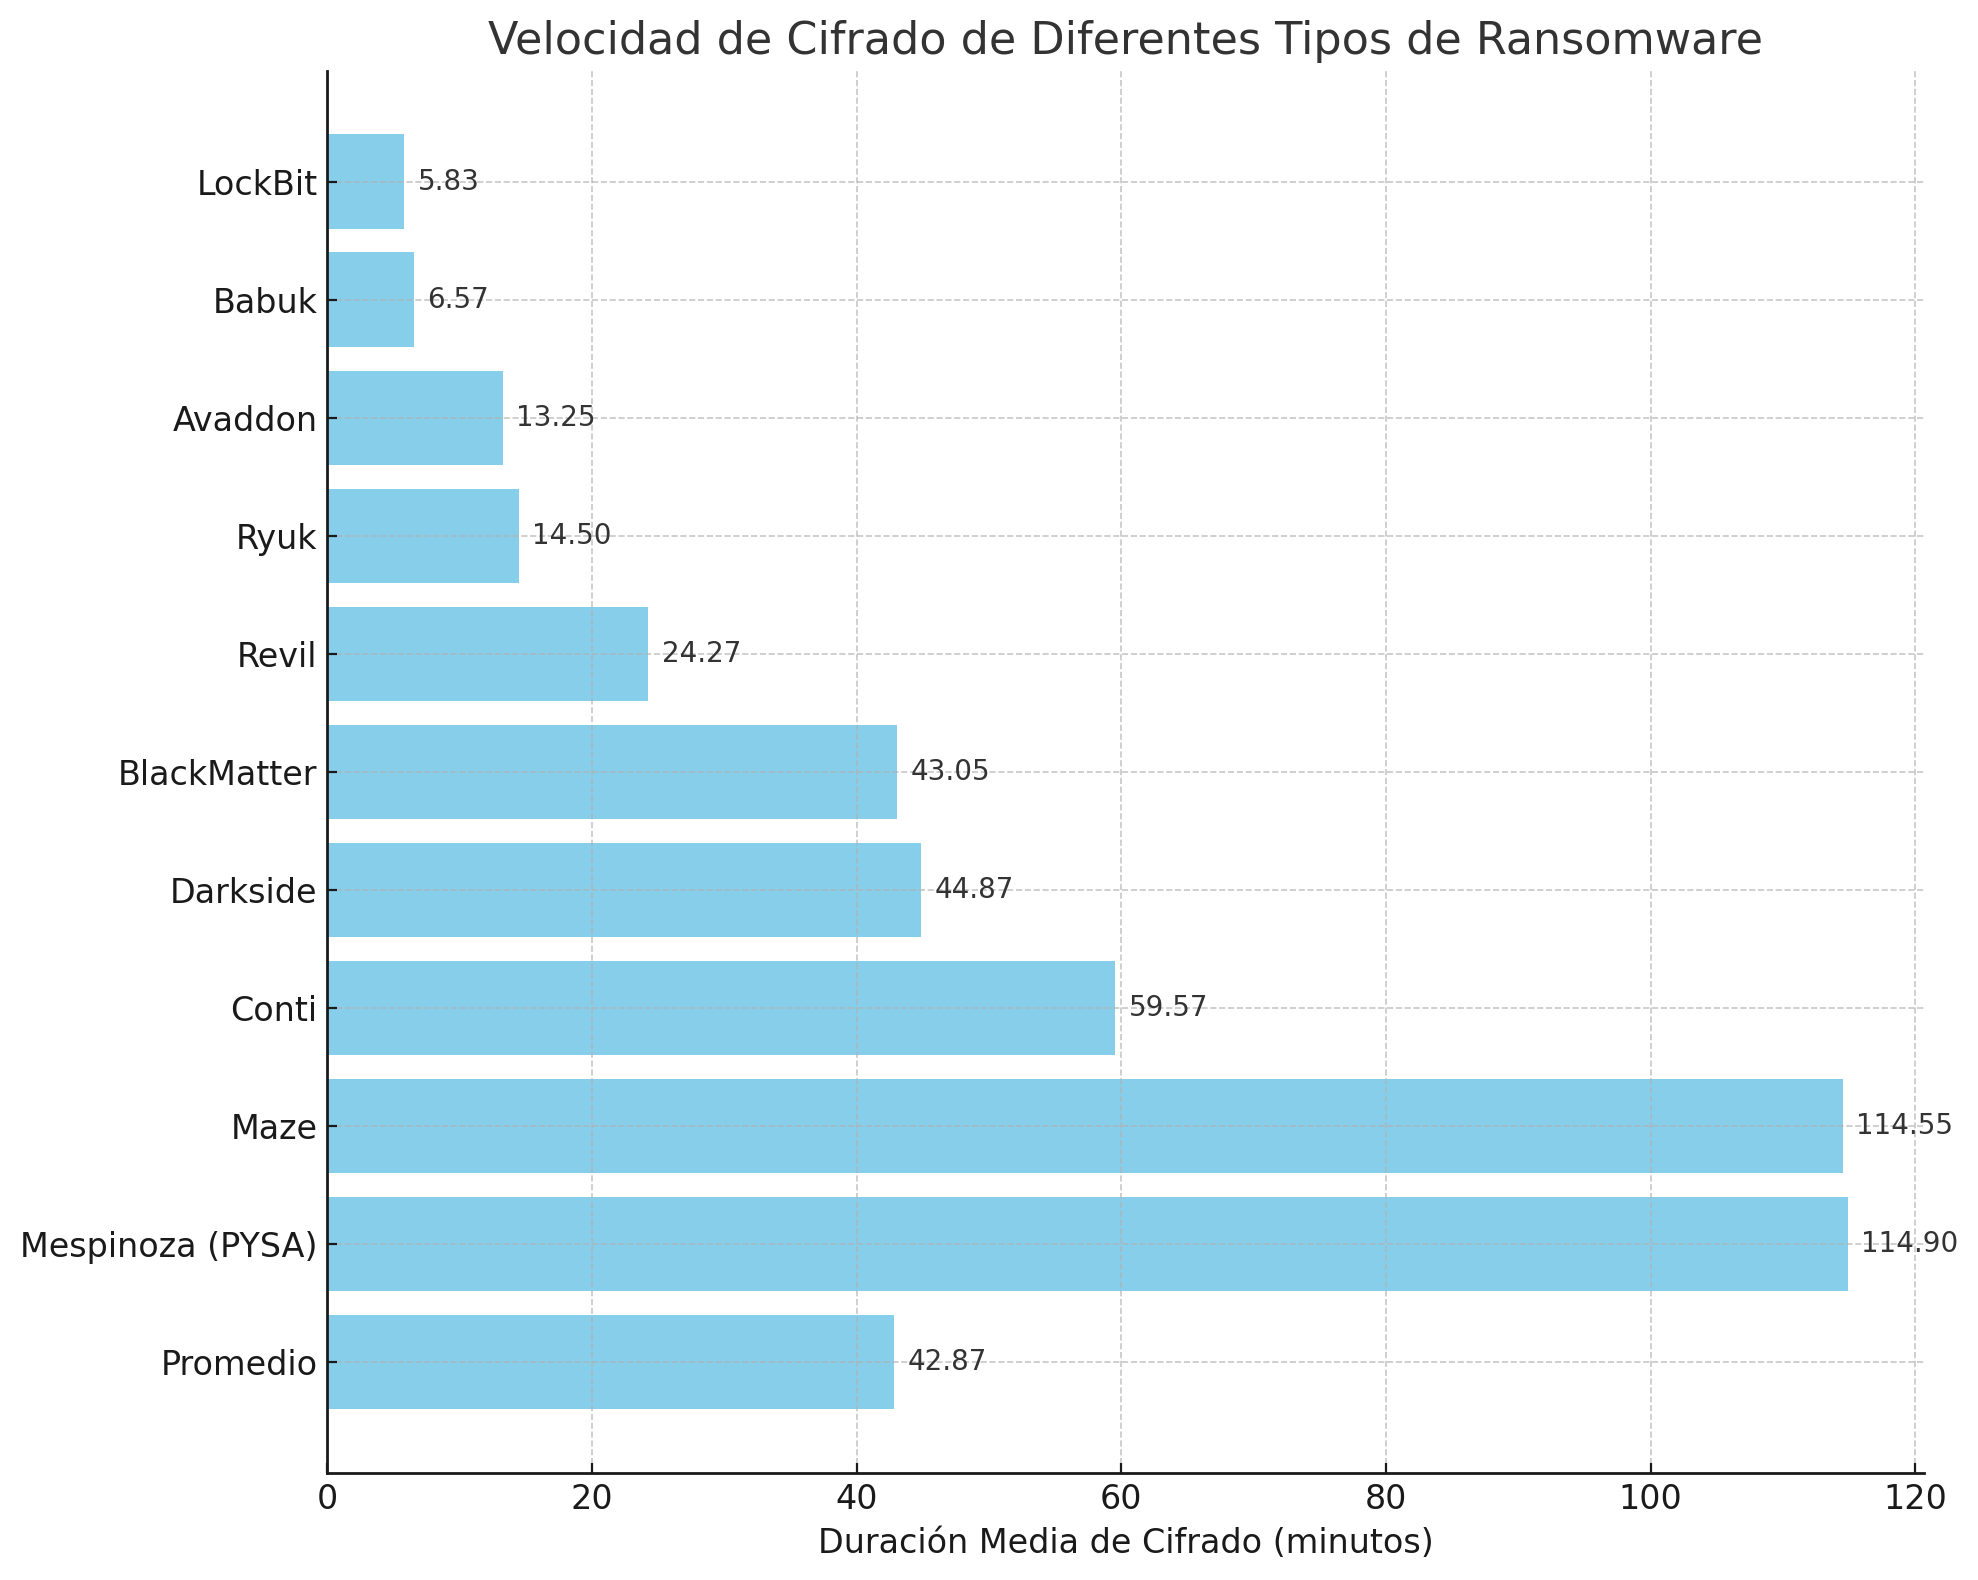
\includegraphics[width=0.8\textwidth]{imagenes/graficos/velocidad_cifrado.png} % Ajusta el nombre de archivo y la escala según sea necesario
    \caption{Comparativa de la velocidad de cifrado de distintas familias de ransomware. Este gráfico ilustra la duración media de cifrado para cada familia, destacando la eficiencia relativa de sus mecanismos de cifrado. Datos adaptados de un análisis comparativo de velocidades de cifrado de ransomware publicado por Splunk.\autocite{SplunkRansomwareSpeed}}
    \label{fig:mi-grafico}
\end{figure}